\documentclass{note}
\usepackage[cpp,table,pseudo]{mypackage}
\usepackage{footnote}
\usepackage{forest}
\makesavenoteenv{tabular}
\usetikzlibrary{automata,backgrounds,fit,shapes,positioning}

\tikzset{->, % makes the edges directed
>=stealth, % makes the arrow heads bold
node distance=2cm, % specifies the minimum distance between two nodes. Change if necessary.
every state/.style={thick, fill=gray!10}, % sets the properties for each 'state' node
}

\renewcommand{\thefootnote}{\fnsymbol{footnote}}

\title{编译原理笔记}
\author{陈鸿峥}
\date{{\builddatemonth\today}\protect\footnote{\text{Build \builddate\today}}} % protect!

\begin{document}

\maketitle
\renewcommand{\thefootnote}{\arabic{footnote}}
\setcounter{footnote}{0}

\setcounter{tocdepth}{2}%设置深度
\tableofcontents

\bigskip\bigskip

% !TEX root = main.tex

\section{计算机网络概述}
计算机网络将终端设备连接起来并可以传输数据。

\subsection{网络连接方式}
\begin{enumerate}
\item 直接连接的网络(直连网)
\begin{itemize}
\item \underline{点对点(point-to-point)网络}:包括专用介质(dedicated medium)、节点/主机
\begin{itemize}
	\item 单向(simplex):如广播、电视
	\item 半双工(half duplex):异步双向,如对讲机
	\item 全双工(full duplex):同步双向,如电话
\end{itemize}
\item \underline{多路访问(multiple access)网络}:共享介质(shared medium),会产生碰撞(collision)
\begin{itemize}
	\item 单播(unicast):一对一
	\item 多播(multicast):一对多
	\item 广播(broadcast):一对所有
\end{itemize}
\end{itemize}
\item 间接连接的网络:涉及交换机、路由器
\end{enumerate}

\subsection{因特网}
用路由器或网关(gateway)连接起来构成的网络称为互\textred{连}网络(internetwork)。

因特网/互联网(Internet)是一种互连网络,可以看作是把世界各地的广域网互连的网络,是世界上最大的特定计算机网络,采用\textemph{TCP/IP协议簇}作为通信规则。
\begin{itemize}
	\item 系统域网(System Area Network, SAN):电脑、鼠标、USB
	\item 局域网(Local Area Network, LAN):某一区域内由多台计算机互联成的计算机组,一般是方圆几千米以内,如小型实验室;常用\textemph{多路访问网络}
	\item 城域网(Metropolitan Area Network, MAN)
	\item 广域网(Wide Area Network, WAN):\textemph{因特网}
\end{itemize}

\myhline
因特网设备:
\begin{itemize}
	\item 终端系统/主机(end system):运行网络应用程序,如手机、浏览器
	\item 通信链路(communication link):光纤、铜线、无线电、卫星等
	\item 路由器(router):用于连接多个网络形成更大的网络
\end{itemize}

\myhline
因特网的组成:ISP(Internet Service Provider)
\begin{itemize}
	\item 网络边界(network edge):主机及网络程序,终端设备可以通过本地ISP或区域ISP连接上互联网
	\item 接入网络/接入网(access network):有线或无线接入,连接订阅者和服务提供商,如WiFi
	\item 网络核心/主干网(core network):顶层ISP(中国电信、中国移动、中国网通),可以连接局部提供商
\end{itemize}

\subsection{网络服务}
通信服务类型:
\begin{itemize}
	\item 可靠/不可靠:会不会丢包/收发是否完全相同,如文件(可靠)/视频(不可靠)
	\item 面向连接/无连接:需不需要建立通信线路,如电话(连接,双方都要在)/寄信、因特网(无连接,对方可能不在)
	\item 有确认/无确认:需不需要确认对方是否收包,因特网不需要
	\item 请求响应/消息流服务:有请求才有响应/一直发消息,如电视
\end{itemize}

因特网是\textemph{数据报服务},\textemph{无连接无确认(尽力服务)}。

\subsection{因特网体系结构}
因特网体系结构包括以下这\textemph{五层},而ISO/OSI(open system interconnection)网络包括七层协议\footnote{也有TCP/IP四层的说法,将物理层和数据链路层合并起来变成物理网络层}:
\begin{itemize}
	\item 应用层:提供对某些专门应用的支持,如\underline{FTP、SMTP、HTTP}
	\item (OSI)表示层(presentationn):提供数据转换服务, 如\underline{加密解密,压缩解压缩,数据格式变换}
	\item (OSI)会话层(session):简化会话实现机制,如\underline{数据流的检查点设置和回滚,多数据流同步}
	\item 传输层:将网络层获得的包在\textemph{进程之间}数据传送(端到端),如\underline{TCP、UDP}
	\item 网络层:\textemph{路由选择},实现在互联网中的数据传送(主机到主机),如\underline{IP协议、路由协议}
	\item 数据链路层:在\textemph{物理网络}中传送\textemph{包}(跳到跳\footnote{一跳(hop)/节点为一个物理设备,即数据链路层只考虑直连网的情况},节点到节点),如\underline{PPP、Ethernet}
	\item 物理层:线上的\textemph{比特}(传送原始比特流)
\end{itemize}
\par 其中\textemph{网络层以下不可靠,以上可靠};防止丢包的机制:\textemph{重发}。
\par 物理层和数据链路层又被称为\underline{物理网络},网络层和传输层被称为\underline{逻辑网络}。

\myhline
协议(protocol):在网络实体(entities)之间传送消息的规则,如消息的格式、收发消息的次序等。

每层传输的数据单元都称为\textemph{包}(packets),都属于某个协议,又被称为\textemph{协议数据单元}(protocol data unit, PDU),包括\textemph{头部/协议控制信息}(potocal control data, PCI)和\textemph{服务数据单元}(service data unit, SDU)两部分。

\begin{minipage}{0.4\linewidth}
\begin{center}
\begin{tikzcd}
\text{应用层Application}\arrow{d}{\text{消息message}}\\
\text{传输层Transport}\arrow{d}{\text{数据段segment}}\\
\text{网络层Network}\arrow{d}{\text{数据报datagram}}\\
\text{链路层Data-link}\arrow{d}{\text{帧frame}}\\
\text{物理层Physical}
\end{tikzcd}
\end{center}
\end{minipage}
\begin{minipage}{0.6\linewidth}
\begin{figure}[H]
	\centering
	\includegraphics[width=\linewidth]{fig/ipencap.png}
\end{figure}
\end{minipage}

\bigskip
下层把上层通过服务访问点(service access point, SAP)传来的SDU用PCI封装为PDU后传给对等实体(peer entity),即实现相同协议的实体。
同一个互连网络中网络层协议需要相同,链路层协议可以不同。

\myhline
\begin{figure}[H]
	\centering
	\includegraphics[width=0.8\linewidth]{fig/network-flow.PNG}
	\caption*{协议栈(stack):发送时封装(encaptulation),接收时拆封。}
\end{figure}

\myhline
\begin{figure}[H]
	\centering
	\includegraphics[width=0.5\linewidth]{fig/protocol_family.png}
	\caption*{协议簇(protocol family)}
\end{figure}

\subsection{网络性能分析}
当一个包到达时如果有空闲缓存则排队等待转发,产生延迟(delay);
如果没有空闲缓存,则丢弃该包,造成丢失(loss)。

包交换网络中的延迟主要有以下四点:
\begin{itemize}
	\item 处理(processing)延迟:查路由,存储转发(store-and-forward)的延迟会很大
	\item 排队(queueing)延迟:依赖于路由器的拥塞程度
	\item 发送/传输(transmission)延迟:\[\text{传输延迟}=\text{包长(bits)}/\text{链路带宽(bps, bit per second)}\]
	指从发送第一个包到发送最后一个包的间隔
	\item 传播(propagation)延迟:指对于一个包来说从发送到接收所需的时间
	\[\text{传播延迟}=\text{物理链路长度}/\text{信号传播速度}\]
\end{itemize}

接收延迟与传播延迟重合。
故忽略掉处理、排队延迟,
\[\text{总延迟(从第一个包被发送到最后一个包被接收的时间)}=\text{传播延迟}+\text{发送延迟}\]

\myhline
\par 往返时间(round trip time, RTT):从源主机到目的主机再返回源主机所花的时间
\par 带宽(bandwidth):一条链路或通道可达到的\textemph{最大}数据传输速率(bps)
\par 吞吐量(thoughput):一条链路或通路\textemph{实际}数据传输速率

\begin{example}
	如果一个长度为$3000$字节的文件用一个数据包从源主机通过一段链路传给了一个交换机,然后再通过第二段链路到达目的主机。
	如果在包交换机的延迟为$2ms$,两条链路上的传播延迟都是$2\times 10^8m/s$,带宽都是$1Mbps$,长度都是$6000km$。
	采用以下三种方式,问这个文件在这两台主机之间的总延迟是多少?
	\begin{enumerate}
		\item 交换机采用存储转发方式
		\item 将文件分成10个数据包,且存储转发
		\item 收到一位转发一位
	\end{enumerate}
\end{example}
\begin{analysis}
	\begin{enumerate}
	\item 因采用存储转发技术,先计算一段的延时,最后乘2。
	\begin{itemize}
	\item 一段的传输延时:$3000B\times 8/10^6bps=24$ms
	\item 一段的传播延时:$6000km/(2\times 10^8m/s)=30$ms
	\item 转发延时:$2$ms
	\end{itemize}
	总时长:$(24+30)\times 2+2=110$ms
	\item 类似1,但是总时长是一个包的传输传播转发延迟,加上剩余包的接收/传输延迟,见下表加粗部分
	\begin{center}
		\begin{tabular}{|c|c|c|c|c|c|}\hline
			包1 & \textemph{传输} & \textemph{传播} & \textemph{接收} & & \\\hline
			包2 &  & 传输 & 传播 & \textemph{接收} & \\\hline
			包3 &  &  & 传输 & 传播 & \textemph{接收} \\\hline
		\end{tabular}
	\end{center}
	\begin{itemize}
		\item 一段的传输延时:$300B\times 8/10^6bps=2.4$ms
		\item 一段的传播延时:$30$ms
		\item 转发延时:$2$ms
	\end{itemize}
	总时长:$(2.4+30)\times 2+2+2.4\times 9=88.4$ms
	\item 同1,但是只用计算一段传输延时,因为1位的转发延迟忽略。
	故总时长:$24+30\times 2=84$ms
\end{enumerate}
\end{analysis}
% !TEX root = main.tex

\section{词法分析}
分离词法分析和语法分析可以简化这两个任务,同时提升编译器的性能与兼容性。

\subsection{基本定义}
\begin{definition}
令牌(token)是一个\underline{令牌名字}与\underline{可选属性值}构成的对;模式(pattern)描述了每个词素(lexeme)要遵循什么规则;而词素(最小意义单位)则是源程序中一连串满足模式的字母,作为令牌的实例化。
\end{definition}
\begin{example}
考虑C语句\\
 \qquad\qquad\verb'printf("Total = %d\n", score);'\\
其中\verb'printf'和\verb'score'是匹配(match)上令牌\textbf{id}模式的词素,而\verb'"Total = %d\n"'是匹配上字面值\textbf{literal}的词素。
\end{example}
简单来讲,令牌是一个更大的概念,是同类词素的集合。
比如一个令牌\textbf{comparison}的样例词素可以有\texttt{<=}和\texttt{!=}。

\begin{definition}[字母表与语言]
字母表(alphabet)$\Sigma$是有限符号(symbol)的集合,如ASCII就是一个字母表。
字符串(string)$s$是从字母表中抽取的有限符号的序列,$|s|$为字符串长度,$\epsilon$为空串。
语言(language)是字符串的可数集合。
\end{definition}
\begin{example}
字母表$\Sigma=\{0,1\}$,则$\{001,1001\}$和$\{\}$都是定义在$\Sigma$上的语言。
\end{example}

\begin{definition}[字符串术语]
前缀(prefix)和后缀(suffix)都可以包括$\epsilon$。
字串(substring)可通过删除任意前缀和任意后缀(包括\textbf{零个})获得。
真(proper)字串则不包含$\epsilon$。
子序列(subsequence)是删除\textbf{零个}或多个\textbf{不一定连续}的字母得到的字符串。
\end{definition}

语言是一种集合,故集合运算也适用于语言。
\begin{table}[H]
\centering
\begin{tabular}{|c|c|}\hline
并集(union) & $L\cup M$\\\hline
连接(concatenation)/交集 & $LM$\\\hline
柯林闭包(Kleene closure) & $L^*=\cup_{i=0}^\infty L^i$\\\hline
正闭包(positive) & $L^+=\cup_{i=1}^\infty L^i$\\\hline
\end{tabular}
\end{table}

\subsection{正则表达式}
\begin{definition}[正则表达式(regular expression, regex)]
正则表达式$r$定义了语言$L(r)$,以递归形式定义:
\begin{enumerate}
	\item 奠基:
	\begin{itemize}
		\item $\epsilon$是正则表达式,即$L(\epsilon)=\{\epsilon\}$
		\item $a\in\Sigma$是正则表达式,即$L(\va)=\{a\}$(这里用斜体代表符号,粗体代表符号对应的正则表达式)
	\end{itemize}
	\item 推论(induction):若$r$和$s$都是正则表达式给出了语言$L(r)$和$L(s)$,则
	\begin{itemize}
		\item $(r)|(s)$是正则表达式,表示$L(r)\cup L(s)$
		\item $(r)(s)$是正则表达式,表示$L(r)L(s)$
		\item $(r)^*$是正则表达式,表示$(L(r))^*$
		\item $(r)$是正则表达式,表示$L(r)$
	\end{itemize}
\end{enumerate}
正则表达式表示的语言叫做正规集。
\end{definition}

有以下运算规定:
\begin{itemize}
	\item 一元运算符${}^*$有最高优先级,左结合
	\item 连接优先级次之,左结合
	\item $|$优先级\textbf{最低},左结合
\end{itemize}

\begin{definition}[正则定义]
$d_i\to r_i$,其中$d_i$都是名字,且各不相同。
每个$r_i$是$\Sigma\cup\{d_1,\ldots,d_{i-1}\}$中符号上的正则表达式。
\end{definition}
\begin{example}
比如C语言的标识符可记为
\[\begin{aligned}
letter\_ &\to A|B|\cdots|Z|a|b|\cdots|z|\_\\
digit &\to 0|1|\cdots|9\\
id &\to letter\_(letter\_|digit)^*
\end{aligned}\]
\end{example}

正则表达式的拓展\footnote{更多可参见\href{https://regex101.com/}{Regex101}}:
\begin{itemize}
	\item $r^+$代表一个或多个
	\item $r?$代表零或一个
	\item $[a-z]$字母类
\end{itemize}

\subsection{有限自动机}
\subsubsection{确定性/非确定性有限自动机}
确定有限自动机(DFA)不可对$\epsilon$进行移动,而且对于每一状态$s$,输入符号$a$,只有唯一一条出边标记为$a$;而非确定性有限自动机(NFA)可能有多种转换路径。
有限状态集$S$,状态$s_0\in S$为初始状态(start/initial),$F\subset S$为终止状态(accepting/final)。
\begin{example}
识别语言$L((a|b)^*abb)$,下面为一个NFA
\begin{center}
% http://madebyevan.com/fsm/
% \begin{tikzpicture}[scale=0.2]
% \tikzstyle{every node}+=[inner sep=0pt]
% \draw [black] (22.6,-23.6) circle (3);
% \draw (22.6,-23.6) node {$0$};
% \draw [black] (34.6,-23.6) circle (3);
% \draw (34.6,-23.6) node {$1$};
% \draw [black] (47.3,-23.6) circle (3);
% \draw (47.3,-23.6) node {$2$};
% \draw [black] (59.5,-23.6) circle (3);
% \draw (59.5,-23.6) node {$3$};
% \draw [black] (59.5,-23.6) circle (2.4);
% \draw [black] (21.277,-20.92) arc (234:-54:2.25);
% \draw (22.6,-16.35) node [above] {$a$};
% \fill [black] (23.92,-20.92) -- (24.8,-20.57) -- (23.99,-19.98);
% \draw [black] (23.923,-26.28) arc (54:-234:2.25);
% \draw (22.6,-30.85) node [below] {$b$};
% \fill [black] (21.28,-26.28) -- (20.4,-26.63) -- (21.21,-27.22);
% \draw [black] (25.6,-23.6) -- (31.6,-23.6);
% \fill [black] (31.6,-23.6) -- (30.8,-23.1) -- (30.8,-24.1);
% \draw (28.6,-24.1) node [below] {$a$};
% \draw [black] (37.6,-23.6) -- (44.3,-23.6);
% \fill [black] (44.3,-23.6) -- (43.5,-23.1) -- (43.5,-24.1);
% \draw (40.95,-24.1) node [below] {$b$};
% \draw [black] (50.3,-23.6) -- (56.5,-23.6);
% \fill [black] (56.5,-23.6) -- (55.7,-23.1) -- (55.7,-24.1);
% \draw (53.4,-24.1) node [below] {$b$};
% \draw [black] (15.4,-23.6) -- (19.6,-23.6);
% \draw (14.9,-23.6) node [left] {$start$};
% \fill [black] (19.6,-23.6) -- (18.8,-23.1) -- (18.8,-24.1);
% \end{tikzpicture}
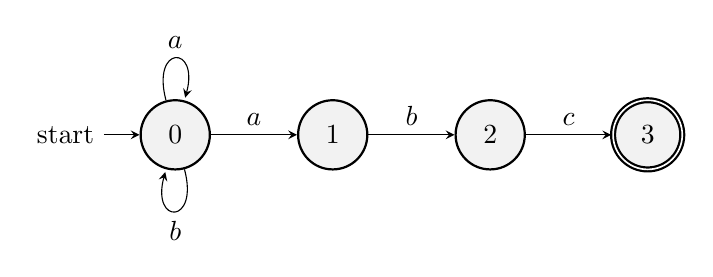
\begin{tikzpicture}
\node[state, initial] (0) {$0$};
\node[state, right of=0] (1) {$1$};
\node[state, right of=1] (2) {$2$};
\node[state, accepting, right of=2] (3) {$3$};
\draw (0) edge[loop above] node{$a$} (0)
(0) edge[loop below] node{$b$} (0)
(0) edge[above] node{$a$} (1)
(1) edge[above] node{$b$} (2)
(2) edge[above] node{$c$} (3);
\end{tikzpicture}
\end{center}
\end{example}

判别字符串能否被DFA识别很简单,只需要读入字符按照状态转移表跳转,判断末态是不是终态即可。
\begin{algorithm}[H]
\centering
\caption{基于DFA的识别算法}
\begin{algorithmic}[1]
\State $s=s_0$
\State $c=nextChar()$
\While{($c$!=\textbf{eof})}
\State $s=move(s,c)$
\State $c=nextChar()$
\EndWhile
\If{$s\in F$}
\State
\Return ``yes''
\Else
\Return ``no''
\EndIf
\end{algorithmic}
\end{algorithm}
时间复杂度为$O(|str|)$。

\subsubsection{正则表达式转NFA}
% https://www3.nd.edu/~kogge/courses/cse30151-fa17/Public/other/tikz_tutorial.pdf

\begin{enumerate}
	\item 奠基
\begin{itemize}
\item 对于表达式$\epsilon$,构建NFA
\begin{center}
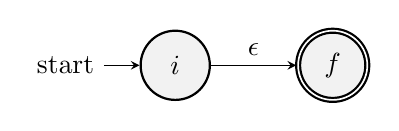
\begin{tikzpicture}
\node[state, initial] (1) {$i$};
\node[state, accepting, right of=1] (2) {$f$};
\draw (1) edge[above] node{$\epsilon$} (2);
\end{tikzpicture}
\end{center}

\item 对于任意子表达式$a\in\Sigma$,构建NFA
\begin{center}
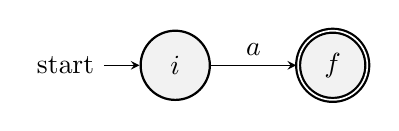
\begin{tikzpicture}
\node[state, initial] (1) {$i$};
\node[state, accepting, right of=1] (2) {$f$};
\draw (1) edge[above] node{$a$} (2);
\end{tikzpicture}
\end{center}
\end{itemize}
	\item 推论
\begin{itemize}
\item $r=s|t$,取并集
\begin{center}
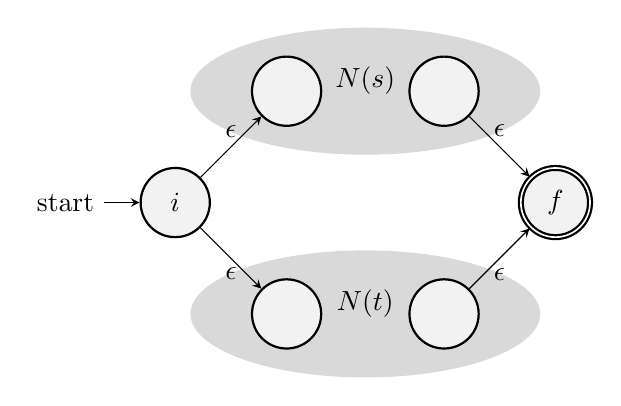
\begin{tikzpicture}
\node[state, initial] (1) {$i$};
\node[state, above right of=1] (2) {};
\node[state, below right of=1] (3) {};
\node[state, right of=2] (4) {};
\node[state, right of=3] (5) {};
\node[state, accepting, below right of=4] (6) {$f$};
\draw (1) edge[above] node{$\epsilon$} (2)
(1) edge[below] node{$\epsilon$} (3)
(4) edge[above] node{$\epsilon$} (6)
(5) edge[below] node{$\epsilon$} (6);
\begin{pgfonlayer}{background}
\node[fit=(2)(4), fill=gray!30, ellipse] {$N(s)$};
\node[fit=(3)(5), fill=gray!30, ellipse] {$N(t)$};
\end{pgfonlayer}
\end{tikzpicture}
\end{center}

\item $r=st$,取连接
\begin{center}
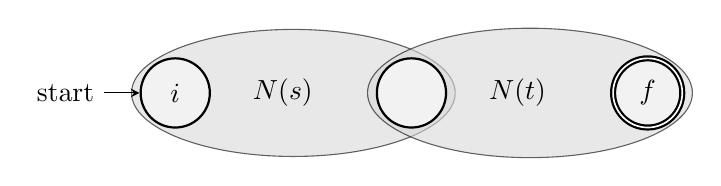
\begin{tikzpicture}[node distance=3cm,
	FIT/.style args = {#1/#2/#3}{ellipse, fill=#1, inner xsep=#2, fit=#3}]
\node[state, initial] (1) {$i$};
\node[state, right of=1] (2) {};
\node[state, accepting, right of=2] (3) {$f$};
\node[right=0.41cm of 1] {$N(s)$};
\node[right=0.41cm of 2] {$N(t)$};
% \draw[draw=gray!30,arrows={->[gray!30]}] (1) edge[above] node{$N(s)$} (2);
% \draw[draw=gray!30,arrows={->[gray!30]}] (2) edge[above] node{$N(t)$} (3);
\begin{pgfonlayer}{background}
\node[FIT=gray!30/-5mm/(1)(2), draw=black, opacity=0.6] {};
\node[FIT=gray!30/-5mm/(2)(3), draw=black, opacity=0.6] {};
\end{pgfonlayer}
\end{tikzpicture}
\end{center}

\item $r=s^*$,Kleene闭包
\begin{center}
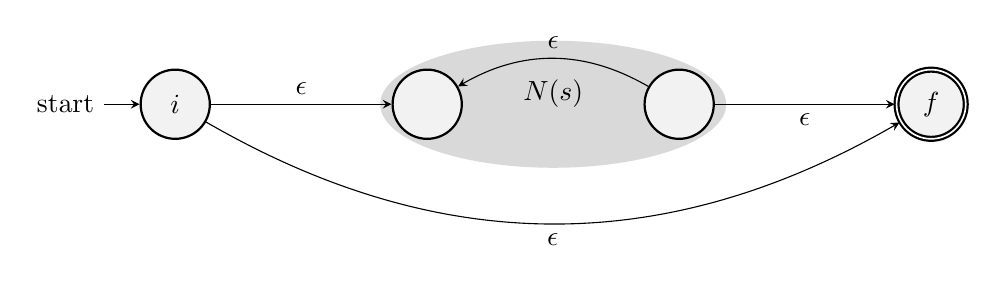
\begin{tikzpicture}[node distance=3.2cm,
	FIT/.style args = {#1/#2/#3}{ellipse, fill=#1, inner xsep=#2, fit=#3}]
\node[state, initial] (1) {$i$};
\node[state, right of=1] (2) {};
\node[state, right of=2] (3) {};
\node[state, accepting, right of=3] (4) {$f$};
\draw (1) edge[above] node{$\epsilon$} (2)
(1) edge[bend right, below] node{$\epsilon$} (4)
(3) edge[above, bend right] node(e){$\epsilon$} (2)
(3) edge[below] node{$\epsilon$} (4);
\begin{pgfonlayer}{background}
\node[FIT=gray!30/-5mm/(2)(3)] {$N(s)$};
\end{pgfonlayer}
\end{tikzpicture}
\end{center}
\end{itemize}
\end{enumerate}

\subsubsection{NFA转DFA}
\begin{definition}[$\epsilon$闭包及$move$]
$\epsilon$闭包是可通过NFA的$\epsilon$边转换的状态。
$move(T,a)$为状态$s\in T$通过输入符号$a$可到达的新的状态。
\end{definition}
\begin{algorithm}[H]
\centering
\caption{子集构造(NFA转DFA)}
\begin{algorithmic}[1]
\Require NFA $N$
\Ensure DFA $D$(与$N$接受相同的语言)
\State $\epsilon$-$closure(s_0)$是$Dstates$的唯一状态,且未被标记(unmarked)
\While{在$Dstates$中还有未被标记的状态$T$}
\State 标记$T$
\For{每一个输入符号$a$}
\State $U=\epsilon$-$closure(move(T,a))$
\If{$U\notin Dstates$}
\State 将$U$作为未标记的状态加入$Dstates$
\EndIf
\State $Dtran[T,a]=U$
\EndFor
\EndWhile
\end{algorithmic}
\end{algorithm}

\begin{example}
考虑以下NFA:
\begin{center}
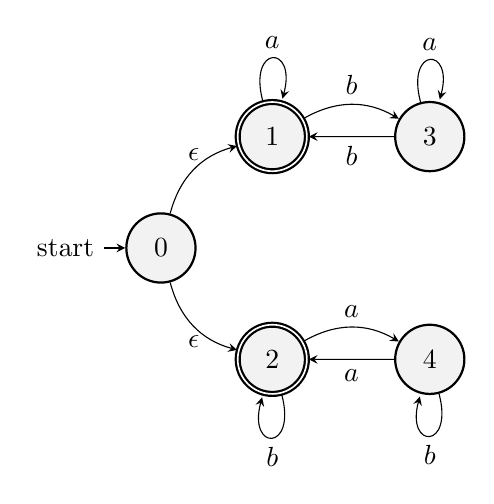
\begin{tikzpicture}[scale=0.6]
\node[state, initial] (0) {0};
\node[state, accepting, above right of=0] (1) {1};
\node[state, right of=1] (3) {3};
\node[state, accepting, below right of=0] (2) {2};
\node[state, right of=2] (4) {4};
\draw (0) edge[bend left, above] node{$\epsilon$} (1)
(0) edge[bend right, below] node{$\epsilon$} (2)
(1) edge[loop above] node{$a$} (1)
(2) edge[loop below] node{$b$} (2)
(1) edge[bend left, above] node{$b$} (3)
(3) edge[below] node{$b$} (1)
(3) edge[loop above] node{$a$} (3)
(2) edge[bend left, above] node{$a$} (4)
(4) edge[below] node{$a$} (2)
(4) edge[loop below] node{$b$} (4);
\end{tikzpicture}
\end{center}
\begin{enumerate}
	\item 这一NFA接受什么语言(用自然语言描述)?
	\item 构造接受同一语言的DFA.
\end{enumerate}
\end{example}
\begin{analysis}
\begin{enumerate}
	\item 含有偶数个$a$或偶数个$b$的由$a$、$b$构成的字符串,或者全是$a$或全是$b$
	\item 由subset construction算法构造如下
\begin{center}
\begin{tabular}{|l|l|l|l|}\hline
NFA & DFA & $a$ & $b$\\\hline
$\{0,\underline{1,2}\}$ & $A$ & $\{1,4\}$ & $\{2,3\}$\\\hline
$\{\underline{1},4\}$ & $B$ & $\{1,2\}$ & $\{3,4\}$\\\hline
$\{\underline{2},3\}$ & $C$ & $\{3,4\}$ & $\{1,2\}$\\\hline
$\{\underline{1,2}\}$ & $D$ & $\{1,4\}$ & $\{2,3\}$\\\hline
$\{3,4\}$ & $E$ & $\{2,3\}$ & $\{1,4\}$\\\hline
\end{tabular}
\end{center}
\begin{center}
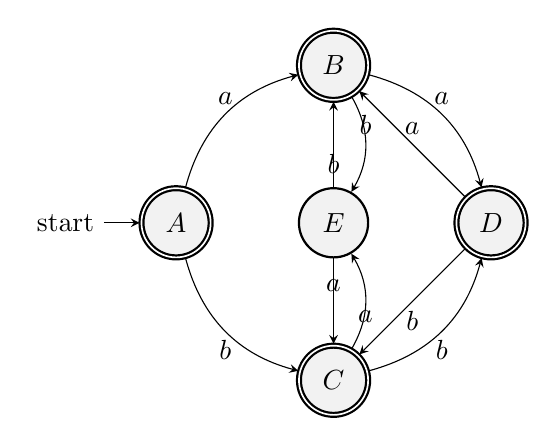
\begin{tikzpicture}
\node[state] (4) {$E$};
\node[state, accepting, initial, left of=4] (0) {$A$};
\node[state, accepting, above of=4] (1) {$B$};
\node[state, accepting, below of=4] (2) {$C$};
\node[state, accepting, right of=4] (3) {$D$};
\draw (0) edge[bend left, above] node{$a$} (1)
(0) edge[bend right, below] node{$b$} (2)
(1) edge[bend left, above] node{$a$} (3)
(1) edge[bend left, above] node{$b$} (4)
(2) edge[bend right, below] node{$a$} (4)
(2) edge[bend right, below] node{$b$} (3)
(3) edge[above] node{$a$} (1)
(3) edge[below] node{$b$} (2)
(4) edge[above] node{$a$} (2)
(4) edge[below] node{$b$} (1);
\end{tikzpicture}
\end{center}
\end{enumerate}
\end{analysis}

直接用NFA识别语言算法如下,需要每次算所有当前\textbf{可能状态}执行动作$c$后的$\epsilon$闭包。
\begin{algorithm}[H]
\centering
\caption{子集构造(NFA转DFA)}
\begin{algorithmic}[1]
\State $S=\epsilon$-$closure(s_0)$
\State $c=nextChar()$
\While{$c$!=\textbf{eof}}
\State $S=\epsilon$-$closure(move(S,c))$
\State $c=nextChar()$
\EndWhile
\If {$S\cap F$!=$\varnothing$}
\State\Return ``yes''
\Else
\State\Return ``no''
\EndIf
\end{algorithmic}
\end{algorithm}

\begin{theorem}
DFA,NFA和正则表达式三者的描述能力是一样的。
\end{theorem}
% !TEX root = main.tex

\section{语法分析}
\subsection{上下文无关法}
语法分析需要解决:从词法分析中获得的每个属性字(token)在语句中承担什么角色,同时检查语句是否符合程序语言的语法。
\begin{definition}[上下文无关法(context-free gramma, CFG)]
包括四部分
\begin{itemize}
	\item 终端符号(terminal)的集合$T$
	\item 非终端符号的集合$N$
	\item 唯一的开始符号$S\in N$
	\item 若干以下形式的产生式(production)
	\[X\to Y_1Y_2\ldots Y_n\]
	其中$X\in N$且$Y_i\in T\cup N\cup\{\epsilon\}$。
	多个左侧相同的产生式右侧可用$\mid$合并。
\end{itemize}
\end{definition}
\begin{definition}[推导(derivation)]
从开始符号开始,每一步推导就是用一个产生式的右方取代左端的非终端符号。
\end{definition}

CFG定义语言的能力比正则表达式强很大原因是它引入了\textbf{递归}的因素。

\begin{example}
用上下文无关文法定义下列语言:
\begin{itemize}
	\item $L=\{0^n1^n\mid n\geq 1\}$:$E\to 0E1\mid 01$
	\item 只含有$0$和$1$的回文串:$S\to 0S0\mid 1S1\mid 0\mid 1\mid \epsilon$
	\item 只含有$($和$)$的匹配括号串:$E\to (E)\mid EE\mid \epsilon$
\end{itemize}
\end{example}

\begin{itemize}
	\item 最左推导:每步推导都替换最左侧的非终端符号
	\[E\xRightarrow{lm}
	-E\xRightarrow{lm}
	-(E)\xRightarrow{lm}
	-(E+E)\xRightarrow{lm}
	-(id+E)\xRightarrow{lm}
	-(id+id)\]
	\item 最右推导:每步推导都替换最右侧的非终端符号
	\[E\implies
	-E\implies
	-(E)\implies
	-(E+E)\implies
	-(E+id)\implies
	-(id+id)\]
\end{itemize}

\begin{definition}[二义性]
如果对于一个文法,存在一个句子,对这个句子可以构造两棵不同的分析树,那么我们称这个文法为二义的。
\end{definition}
看语法分析树的叶子结点能不能连成句子。

\begin{example}
对于文法$E\to E+E\mid E*E\mid -E\mid (E)\mid id$及句子$id+id*id$,有以下两种推导:

\begin{minipage}{0.5\linewidth}
\[\begin{aligned}
E &\implies E+E\\
&\implies id+E\\
&\implies id+E*E\\
&\implies id+id*E\\
&\implies id+id*id\\
\end{aligned}\]
\end{minipage}
\begin{minipage}{0.5\linewidth}
\[\begin{aligned}
E &\implies E+E\\
&\implies id+E\\
&\implies id+E*E\\
&\implies id+id*E\\
&\implies id+id*id\\
\end{aligned}\]
\end{minipage}
\end{example}

文法二义性的消除可通过引入更多的产生式。
\begin{example}
$E\to E+E\mid E*E\mid (E)\mid id$是有二义的,因为不知道应该先算加法还是乘法。
可将其改为
\[\begin{aligned}
E &\to E+T\mid T\\
T &\to T*F\mid F\\
F &\to (E)\mid id
\end{aligned}\]
其中$E$为Expression,$T$为Term,$F$为Facotr,即可消除二义性(必然得先算乘法)。
\end{example}

并不是所有上下文无关文法都可以做到无二义,也无法判断一个上下文无关文法是否是二义的。

\subsection{NFA转CFG}
\begin{enumerate}
	\item 对于NFA的每一状态$i$,创建非终态$A_i$
	\item 若状态$i$在输入$a$上有转换边到状态$j$,则添加生成式$A_i\to aA_j$;
	若状态$i$在输入$\epsilon$上转换到状态$j$,则添加生成时$A_i\to A_j$
	\item 若$i$是接受状态,则添加$A_i\to\epsilon$
	\item 若$i$是初始状态,则令$A_i$为语法的初始符号
\end{enumerate}

\begin{definition}[右线性文法]
如果每个产生式都属于下列形式之一
\[A\to aB\qquad A\to a\qquad A\to\epsilon\]
则这样的文法称为右线性文法
\end{definition}
\begin{definition}[左线性文法]
如果每个产生式都属于下列形式之一
\[A\to Ba\qquad A\to a\qquad A\to\epsilon\]
则这样的文法称为左线性文法
\end{definition}

在处理程序时,上下文无法文法存在局限性,无法解决诸如以下问题:
\begin{itemize}
\item 变量先声明,再使用
\item 调用函数时,实参个数和形参个数一致
\end{itemize}
都得留到语义分析阶段才解决。
% !TEX root = main.tex

\section{语义分析与中间表示}
\begin{itemize}
\item 高层中间表示:语法树、有向无环图(DAG),用于静态类型检查
\item 低层中间表示:三地址码,适合机器相关的任务(寄存器分配、指令选择)
\end{itemize}
\begin{lstlisting}[language=c++]
x = y op z // arithmetic and logical
x = op y  // negation and conversion
x = y // copy
goto L // unconditional jump
if x goto L // conditional jump 
if False x goto L // conditional jump
if x op y goto L // relational operation
param x1 // parameter passing
param x2
...
param xn
call p, n // procedure call
y = call p, n // function call
return y // return a value
x = y[i] // indexed copy, i is the offset
x[i] = y
x = &y // address and pointer assignment
x = *y
*x = y
\end{lstlisting}

\verb'top'指代当前的符号表,\verb'gen'代表生成中间代码,\verb'||'代表代码的连接。
\begin{center}
\begin{tabular}{|l|l|}\hline
$S \to id = E$ & \verb"S.code = E.code || gen(top.get(id.lexeme) '=' E.addr)"\\\hline
$E \to E_1 + E_2$ & \begin{tabular}{l}
\verb'E.addr = new Temp()'\\
\verb"E.code = E1.code || E2.code || gen(E.addr '=' E1.addr '+' E2.addr)"
\end{tabular}\\\hline
$E \to -E_1$ & \begin{tabular}{l}
\verb'E.addr = new Temp()'\\
\verb"E.code = E1.code || gen(E.addr '=' minus E1.addr)"
\end{tabular}\\\hline
$E \to (E_1)$ & \begin{tabular}{l}
\verb'E.addr = E1.addr'\\
\verb"E.code = E1.code"
\end{tabular}\\\hline
$L \to L_1 [E]$ & \begin{tabular}{l}
\verb'L.array = L1.array'\\
\verb"L.type = L1.type.element"\\
\verb"t = new Temp()"\\
\verb"L.addr = new Temp()"\\
\verb"gen(t '=' E.addr '*' L.type.width)"\\
\verb"gen(L.addr '=' L1.addr '+' t)"
\end{tabular}\\\hline
\verb'S'$\to$\verb'if (B) S1 else S2' & \begin{tabular}{l}
\verb'B.true = new Label()'\\
\verb'B.false = new Label()'\\
\verb'S1.next = S2.next = S.next'\\
\verb'S.code = B.code || label(B.true) || S1.code ||'\\
\verb"         gen('goto' S.next) || label(B.false) || S2.code"
\end{tabular}\\\hline
\end{tabular}
\end{center}

三地址码与对应的DAG如下图所示,注意这里将相同终端符号结点都给合并了。

\begin{minipage}{0.5\linewidth}
\[\begin{aligned}
t_1 &= b - c\\
t_2 &= a * t_1\\
t_3 &= a + t_2\\
t_4 &= t_1 * d\\
t_5 &= t_3 + t_4
\end{aligned}\]
\end{minipage}
\begin{minipage}{0.5\linewidth}
\begin{figure}[H]
\centering
\includegraphics[width=0.5\linewidth]{fig/three-addr-code-dag.jpg}
\end{figure}
\end{minipage}

\begin{example}
令\verb'a'表示一个$2\times 3$的整型数组,\verb'b'表示一个$3\times 4$的整型数组.
假定一个整数的宽度为$4$.
试使用课本图6.22的翻译模式,翻译赋值语句\verb'x=a[i][j]+b[i][j]'.
提示:参考课本例6.12.
\end{example}
\begin{analysis}
带注释的分析树如下
\begin{center}
\scalebox{0.8}{
\begin{forest}
sn edges
[{$S$}
	[{$x$}]
	[{$=$}]
	[{$E.addr=t_9$}
		[{$E.addr=t_4$}
			[{\begin{tabular}{l}$L.array=a$\\ $L.type=int$\\ $L.addr=t_3$\end{tabular}}
				[{\begin{tabular}{l}$L.array=a$\\ $L.type=array(3,int)$\\ $L.addr=t_1$\end{tabular}}
					[{\begin{tabular}{l}$a.type=$\\$array(2,array(3,int))$\end{tabular}}]
					[{$[$}]
					[{$E.addr=i$}
						[{$i$}]
					]
					[{$]$}]
				]
				[{$[$}]
				[{$E.addr=j$}
					[{$j$}]
				]
				[{$]$}]
			]
		]
		[{$+$}]
		[{$E.addr=t_8$}
			[{\begin{tabular}{l}$L.array=b$\\ $L.type=int$\\ $L.addr=t_7$\end{tabular}}
				[{\begin{tabular}{l}$L.array=b$\\ $L.type=array(4,int)$\\ $L.addr=t_5$\end{tabular}}
					[{\begin{tabular}{l}$b.type=$\\$array(3,array(4,int))$\end{tabular}}]
					[{$[$}]
					[{$E.addr=i$}
						[{$i$}]
					]
					[{$]$}]
				]
				[{$[$}]
				[{$E.addr=j$}
					[{$j$}]
				]
				[{$]$}]
			]
		]
	]
]
\end{forest}
}
\end{center}

生成的三地址码如下
\begin{center}
\begin{tabular}{l}
$t_1 = i * 12$\\
$t_2 = j * 4$\\
$t_3 = t_1 + t_2$\\
$t_4 = a[t_3]$\\
$t_5 = i * 16$\\
$t_6 = j * 4$\\
$t_7 = t_5 + t_6$\\
$t_8 = b[t_7]$\\
$t_9 = t_4 + t_8$\\
$x   = t_9$
\end{tabular}
\end{center}
\end{analysis}
% !TEX root = main.tex

\section{运行时系统}
\subsection{存储管理}
\begin{figure}[H]
\centering
\includegraphics[width=0.5\linewidth]{fig/stack.jpg}
\end{figure}

\subsection{垃圾回收}
\begin{itemize}
	\item 引用计数(reference counting):创建加1,删除减1
	\begin{itemize}
		\item 简单、立即增量式回收
		\item 不能回收循环引用的示例
	\end{itemize}
	\begin{figure}[H]
	\centering
	\includegraphics[width=0.8\linewidth]{fig/reference_counting.jpg}
	\end{figure}
	\item 标记扫除(mark and sweep):做图深搜找连通块
	\begin{itemize}
		\item 有办法清除循环引用
		\item 大量垃圾时效率低,无法满足实时应用
	\end{itemize}
	\item 标记压缩(mark and compact):标记,计算新地址,拷贝对象到新地址并更新引用
	\begin{figure}[H]
	\centering
	\includegraphics[width=0.8\linewidth]{fig/mark_and_compact.jpg}
	\end{figure}
	\item 拷贝收集(copying collector):堆被划分为两个区域,可达对象一旦被发现就会立即被移动,但不可达对象不做改动
	\begin{figure}[H]
	\centering
	\includegraphics[width=0.8\linewidth]{fig/copying_collector.jpg}
	\end{figure}
\end{itemize}

JVM采用了两代(young \& old)的方式,对于年轻的对象采用拷贝收集,对于老的对象则采用标记压缩。
% !TEX root = main.tex

\section{代码生成及优化}
\subsection{代码生成}
\begin{itemize}
	\item 指令选择:选择最适合目标机器的指令来实现IR
	\item 寄存器分配和指派
	\item 指令调度
\end{itemize}

\begin{definition}[基本块(basic block)]
单一入口单一出口。
成为leader的指令:
\begin{enumerate}
	\item 第一条三地址指令
	\item 条件或无条件跳转指令的目标
	\item 条件或无条件跳转指令的下一指令
\end{enumerate}
\end{definition}

\begin{example}
考虑以下基本块:
\[\begin{aligned}
t_0 &= 5\\
t_1 &= 3 * t_0\\
t_2 &= R + r\\
t_3 &= t_1 * t_2\\
t_4 &= t_2\\
t_5 &= t_3 - t_4\\
t_6 &= t_1 * t_2\\
A   &= t_6 + t_5\\
B   &= A - r\\
t_7 &= t_1\\
B   &= t_7 + B
\end{aligned}\]
\begin{enumerate}
\item 构造这一基本块的DAG.
\item 假设只有$A$和$B$在基本块后面还要被引用,产生优化后的三地址代码.
\end{enumerate}
\end{example}
\begin{analysis}
\begin{enumerate}
	\item 基本块的DAG如下图所示
	\begin{figure}[H]
	\centering
	\includegraphics[width=0.3\linewidth]{fig/dag-1.pdf}
	\end{figure}
	\item 由于只有$A$和$B$在基本块后面还要被引用,因此最终只需保留$A$和$B$的结果即可。
	无依赖关系的代码都可以作为死代码优化删除。
	最终优化后的三地址代码如下
\[\begin{aligned}
t_2 &= R + r\\
t_3 &= 15 * t_2\\
t_5 &= t_3 - t_2\\
A &= t_3 + t_5\\
B &= A - r\\
B &= 15 + B
\end{aligned}\]
\end{enumerate}
\end{analysis}

\subsection{代码优化}
\begin{itemize}
	\item 窥孔优化(peephole):基于滑动窗口,最小粒度
\begin{lstlisting}[language=c++]
x = x + 0 // eliminated
x = x * 1 // eliminated
y = x * 2 // y = x << 1
LD R0, a
ST a, R0 // eliminated
\end{lstlisting}
	\item 局部优化:在基本块内的优化
\begin{itemize}
	\item 公共子表达式删除
	\item 常量/拷贝传递
	\item 荣誉操作消除
\end{itemize}
	\item 循环优化:在循环内的优化
	\item 全局优化:最粗粒度的优化
\end{itemize}

\begin{definition}[循环(loop)]
只有唯一入口/头的强连通子图
\end{definition}

\begin{example}
考虑下列代码片段:
\begin{enumerate}[label=(\arabic*)]
\item \verb'm := 0'
\item \verb'v := 0'
\item \verb'if v >= n goto (19)'
\item \verb'r := v'
\item \verb's := 0'
\item \verb'if r < n goto (9)'
\item \verb'v := v + 1'
\item \verb'goto (3)'
\item \verb's := v + r'
\item \verb'y := 0 * x'
\item \verb'z := v - y'
\item \verb'x := z + r'
\item \verb'r := m - x'
\item \verb'if s <= m goto (17)'
\item \verb'm := s'
\item \verb's := s + r'
\item \verb'r := r+1'
\item \verb'goto (6)'
\item \verb'return m'
\end{enumerate}
为这段代码划分基本块(Basic Block),并画出控制流图(Control Flow Graph).
在答案中你可以直接画出控制流图,但对图中的每个结点,请用$m\thicksim n$表示相应的基本块由第$m$至第$n$条语句组成.
\end{example}
\begin{analysis}
如下图所示,共$9$个基本块,每个基本块包含的语句已在图中标出。
\begin{figure}[H]
\centering
\includegraphics[width=0.7\linewidth]{fig/dag-2.pdf}
\end{figure}
\end{analysis}

\end{document}